\documentclass[a4paper]{article}

\usepackage[svgnames]{xcolor}
\usepackage[font=small,format=plain,labelfont=bf,up,textfont=up]{caption}
\usepackage{fancyvrb}
\usepackage[margin=2cm]{geometry}
\usepackage{graphicx}
\usepackage{hyperref}
\usepackage{minted}
\usepackage{siunitx}
\usepackage{tikz}
\usepackage{todonotes} % Only for drafting

\usetikzlibrary{positioning,shapes}

% Args are module name, filename, caption text
\newcommand{\modulelisting}[3]{
  \begin{listing}[p]
    \linespread{.9}\inputminted[fontsize=\scriptsize,linenos]{systemverilog}{#2}
    \caption{#3}
    \label{lst:#1}
  \end{listing}
}

% Args are module name, caption text
\newcommand{\waveformfigure}[3]{
  \begin{figure}[p]
    \centering\includegraphics[width=\textwidth]{assets/#1}
    \caption{#2}
    \label{fig:#1}
  \end{figure}
}

\title{ELEC2221 D1: Design and test of a sequential multiplier}
\author{Kier Davis \\
Username: kad2g15 \\
Course: MEng Electronic Engineering \\
Tutor: Dr. Klaus-Peter Zauner \\
Lab group: F17 \\
Lab session: November 21, 2016}

\begin{document}

\maketitle

\begin{abstract}
  % Implemented multiplier
  % Simulated in ModelSim, with assertions
  % Synthesised for MachXO2 using Synplify, tested
  % Extensions: debouncer, 8-bit
  \todo[inline]{blah}
\end{abstract}

\section{Adder design, simulation and synthesis}
\label{sec:adder}

The adder was implemented as an integrated part of the \texttt{multiplier\_datapath} module. It takes as inputs the current state of the \texttt{a} register and a signal named \texttt{addend}, and produces a 4-bit \texttt{sum} and a 1-bit \texttt{carry}. The value of \texttt{addend} is chosen based on the state of the least significant bit of \texttt{q}. If this bit is zero, \texttt{addend} is set to zero, and so the output of the adder is equal to \texttt{a}; that is, no actual addition is performed. If, however, the LSB of \texttt{q} is one, \texttt{addend} is set to \texttt{multiplicand}, and so the output of the adder is the sum of \texttt{a} and \texttt{multiplicand}.

\subsection{Implementation}
\label{sec:adder:impl}

The adder itself is implemented on line 72 of Listing~\ref{lst:multiplier_datapath}, and the multiplexer that produces the \texttt{addend} is implemented on line 70.

\subsection{Simulation}
\label{sec:adder:sim}

The adder was not simulated on its own, but only as a part of \texttt{multiplier\_datapath}; see Section~\ref{sec:reg:sim} for further details.

It can be seen from the results of running the simulation of \texttt{multiplier\_datapath} in ModelSim (illustrated in Figure~\ref{fig:test_multiplier_datapath}) that at the clock edge occurring at time \SI{8000}{\milli\second}, the value of the \texttt{product} signal changes from \texttt{0101 1001} to \texttt{1000 0100}. \texttt{product} is simply the concatenation of the \texttt{a} and \texttt{q} registers, so \texttt{a} must change from \texttt{0101} to \texttt{1000} and \texttt{q} must change from \texttt{1001} to \texttt{0100}. This is consistent with the results obtained by working through the method by hand:

\vspace{10pt}
\begin{tabular}{ll}
\mintinline{text}{  0101 1001} & Initial values of a and q \\
\mintinline{text}{+ 1011     } & Addend = multiplicand (1011), since LSB of q is 1 \\
\mintinline{text}{------     } & \\
\mintinline{text}{1 0000     } & Sum and carry \\
\mintinline{text}{1 0000 1001} & Same as first line, but with a replaced by sum/carry \\
\mintinline{text}{  1000 0100} & Resulting of shifting previous line right by one place \\
\end{tabular}
\vspace{10pt}

This transition, and all other transitions of the \texttt{product} signal, are verified by assertions in the simulation.

\subsection{Synthesis}
\label{sec:adder:synth}

The adder was synthesised as part of the \texttt{multiplier\_datapath} module; see Section~\ref{sec:reg:synth} for further details.

\section{Register design, simulation and synthesis}
\label{seg:reg}

The registers were implemented in the \texttt{multiplier\_datapath} module, together with the adder/shifter.

The \texttt{multiplier\_datapath} module has two 4-bit data inputs, \texttt{multiplicand} and \texttt{multiplier}. These are the two input numbers to the multiplier, and are equivalent to \texttt{M} and \texttt{Qin} respectively in the sample code. Similarly, there is one 8-bit data output, \texttt{product}, which is equivalent to \texttt{AQ} in the sample code.

The module takes two control signals, \texttt{do\_init} and \texttt{do\_shift}, in addition to the clock and asynchronous reset signals. If \texttt{do\_init} is asserted during a rising clock edge, the \texttt{a} and \texttt{q} registers are loaded with their initial values (0 and \texttt{multiplier} respectively). If \texttt{do\_shift} is asserted during a rising clock edge, then \texttt{multiplicand} is conditionally added to \texttt{a}, and then \texttt{a} and \texttt{q} are shifted right by one place, completing one iteration of the multiplication algorithm in a single clock cycle.

\subsection{Implementation}
\label{sec:reg:impl}

The source code of the \texttt{multiplier\_datapath} module is given in Listing~\ref{lst:multiplier_datapath}.

\modulelisting{multiplier_datapath}{../src/multiplier/multiplier_datapath.sv}
  {Source code of the \texttt{multiplier\_datapath} module, which contains the data registers $a$ and $q$ and the add/shift computation logic.}

\subsection{Simulation}
\label{sec:reg:sim}

A testbench for the \texttt{multiplier\_datapath} module was prepared. Its source code is given in Listing~\ref{lst:test_multiplier_datapath}. The testbench was then simulated using ModelSim, giving the waveform diagram shown in Figure~\ref{fig:test_multiplier_datapath}. After correcting some minor syntax errors, the testbench and the module under test worked first time, without any assertions failing.

The testbench begins with the reset signal active, and checks that the registers \texttt{a} and \texttt{q} (whose values are concatenated to form the signal \texttt{product}) are reset to zero. It then releases the system from reset, and asserts the \texttt{do\_init} for one clock cycle, checking that \texttt{q} is set to 6, the value arbitrarily chosen for the second multiplier input. It then asserts \texttt{do\_shift} for four of the five following clock cycles, checking the state of the registers at each stage. The results of these operations can be observed in Figure~\ref{fig:test_multiplier_datapath}.

\modulelisting{test_multiplier_datapath}{../src/multiplier/test/test_multiplier_datapath.sv}
  {Source code of the \texttt{test\_multiplier\_datapath} module, which tests the operation of the data registers and add/shift computation logic.}

\waveformfigure{test_multiplier_datapath}{Waveform of the \texttt{test\_multiplier\_datapath} testbench. Values shown in the waveform traces are in hexadecimal.}

\subsection{Synthesis}
\label{sec:reg:synth}

\todo[inline]{todo}

\section{Sequencer design, simulation and synthesis}
\label{sec:seq}

The multiplier is controlled by an algorithmic state machine (ASM), which is implemented in the \texttt{multiplier\_controller} module. It uses an auxillary 2-bit counter to store the number of remaining cycles of the shift/add operation. This counter has two control signal inputs, \texttt{do\_preset} and \texttt{do\_decrement}. \texttt{do\_preset} causes the value of the counter to its maximum value (3) on the next clock cycle, while \texttt{do\_decrement} causes the value of the counter to be decreased by 1 on the next clock cycle. It has only one output, \texttt{is\_zero}, which is high if the counter is equal to zero.

The state machine, illustrated in Figure~\ref{fig:asm}, has three states named Idle, Working and Done. The system begins in the Idle state. When the \texttt{start} signal goes high, the system moves to the Working state. On this transition, the \texttt{a} and \texttt{q} registers are initialised by setting the datapath's \text{do\_init} signal high, and the counter is set to its maximum value by settings its \texttt{do\_preset} signal high.

While in the Working state, the datapath's \texttt{do\_shift} control input is held high, causing the \texttt{a} and \texttt{q} registers to be continually shifted and added. The state of the \texttt{is\_zero} signal is checked on each clock cycle; if it is high, then the system moves to the Done state, else it decreases the value of the counter by one by asserting the \texttt{do\_decrement} signal. Since \texttt{do\_shift} is still asserted when the counter's value is zero, it will be high for four clock cycles in a row, resulting in four iterations of the shift/add operation being applied to the \texttt{a} and \texttt{q} registers.

In the Done state, the system holds the \texttt{ready} output high, signalling the end of computation. It waits for the \texttt{start} input to go low again before transitioning back to the Idle state.

\begin{figure}[p]
  \centering
  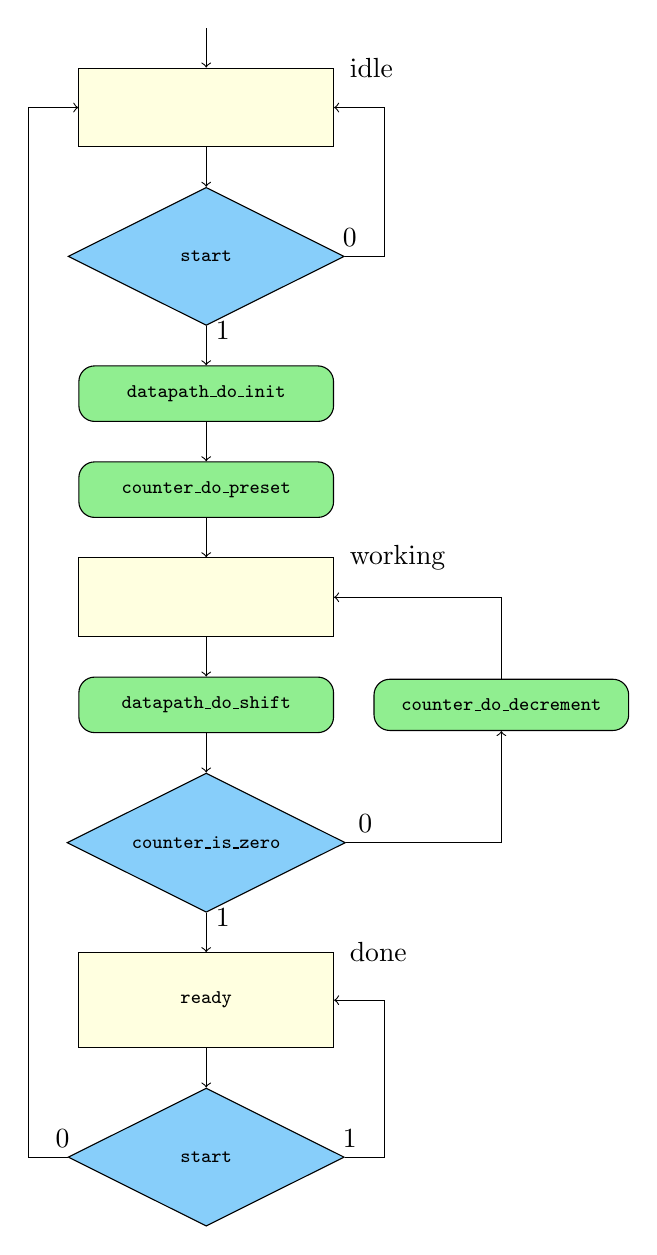
\begin{tikzpicture}[->,
                      node distance=.5cm and .5cm,
                      basenode/.style={draw,text width=3cm,text centered,inner ysep=.25cm,font={\scriptsize}},
                      state/.style={basenode,rectangle,inner ysep=.5cm,fill=LightYellow},
                      decision/.style={basenode,diamond,aspect=2,inner ysep=0cm,fill=LightSkyBlue},
                      condout/.style={basenode,rectangle,rounded corners=.2cm,fill=LightGreen}]
    \node[coordinate] (begin) {start};
    \node[state,label={[anchor=west,xshift=1.7cm]90:idle}] (idle) [below=of begin] {};
    \node[decision] (idle-start) [below=of idle] {\texttt{start}};
    \node[condout] (idle-datapath) [below=of idle-start] {\texttt{datapath\_do\_init}};
    \node[condout] (idle-counter) [below=of idle-datapath] {\texttt{counter\_do\_preset}};
    \node[state,label={[anchor=west,xshift=1.7cm]90:working}] (working) [below=of idle-counter] {};
    \node[condout] (working-datapath) [below=of working] {\texttt{datapath\_do\_shift}};
    \node[decision] (working-is-zero) [below=of working-datapath] {\texttt{counter\_is\_zero}};
    \node[state,label={[anchor=west,xshift=1.7cm]90:done}] (done) [below=of working-is-zero] {\texttt{ready}};
    \node[decision] (done-start) [below=of done] {\texttt{start}};
    \node[coordinate] (n1) [right=of idle-start] {};
    \node[coordinate] at (idle -| n1) (n0) {};
    \node[condout] (working-counter) [right=of working-datapath] {\texttt{counter\_do\_decrement}};
    \node[coordinate] at (working -| working-counter) (n2) {};
    \node[coordinate] at (working-is-zero -| working-counter) (n3) {};
    \node[coordinate] (n5) [right=of done-start] {};
    \node[coordinate] at (done -| n5) (n4) {};
    \node[coordinate] (n7) [left=of done-start] {};
    \node[coordinate] at (idle -| n7) (n6) {};
    \draw (begin) -> (idle);
    \draw (idle) -> (idle-start);
    \draw (idle-start) -> node[right,very near start] {1} (idle-datapath);
    \draw (idle-datapath) -> (idle-counter);
    \draw (idle-counter) -> (working);
    \draw (working) -> (working-datapath);
    \draw (working-datapath) -> (working-is-zero);
    \draw (working-is-zero) -> node[right,very near start] {1} (done);
    \draw (done) -> (done-start);
    \draw (idle-start) -- node[above,very near start] {0} (n1) -- (n0) -> (idle);
    \draw (working-is-zero) -- node[above,very near start] {0} (n3) -> (working-counter);
    \draw (working-counter) -- (n2) -> (working);
    \draw (done-start) -- node[above,very near start] {1} (n5) -- (n4) -> (done);
    \draw (done-start) -- node[above,very near start] {0} (n7) -- (n6) -> (idle);
  \end{tikzpicture}
  \caption{An ASM chart representing the operation of the multiplier. Rectangular nodes represent states, and arrows represent possible transition paths. The text inside each state node lists the unconditional outputs that are active during that state; the name of the state is instead given by the label at the top-right corner of the node. Rounded rectangles represent conditional outputs that should be asserted only when the transition path is taken. Diamonds represent decisions (input tests).}
  \label{fig:asm}
\end{figure}

\subsection{Implementation}
\label{sec:seq:impl}

The 2-bit counter used for counting the number of remaining iterations of the shift/add operation is implemented in the \texttt{multiplier\_counter} module, whose source code is given in Listing~\ref{lst:multiplier_counter}. The remainder of the state machine is implemented in the \texttt{multiplier\_controller} module, whose source code is given in Listing~\ref{lst:multiplier_controller}. After cleaning up some minor syntax errors, the simulation ran first time with all assertions passing.

\modulelisting{multiplier_counter}{../src/multiplier/multiplier_counter.sv}
  {Source code of the \texttt{multiplier\_counter} module, which contains the 2-bit counter that records the number of remaining iterations of the algorithm.}

\modulelisting{multiplier_controller}{../src/multiplier/multiplier_controller.sv}
  {Source code of the \texttt{multiplier\_controller} module, which contains the state machine that controls the multiplier's operation.}

\subsection{Simulation}
\label{sec:seq:sim}

A testbench for the counter was prepared; its source code is given in Listing~\ref{lst:test_multiplier_counter}. Running this testbench through ModelSim gives the waveform shown in Figure~\ref{fig:test_multiplier_counter}.

\modulelisting{test_multiplier_counter}{../src/multiplier/test/test_multiplier_counter.sv}
  {Source code of the \texttt{test\_multiplier\_counter} testbench, which tests the 2-bit counter used to keep track of the remaining number of iterations.}

\waveformfigure{test_multiplier_counter}{Waveform of the \texttt{test\_multiplier\_counter} testbench. Values shown in the waveform traces are in hexadecimal.}

\subsection{Synthesis}
\label{sec:seq:synth}

\todo[inline]{todo}

\section{Multiplier design, simulation and synthesis}
\label{sec:mult}

The \texttt{multiplier} module encapsulates the \texttt{multiplier\_datapath}, \texttt{multiplier\_counter} and \texttt{multiplier\_controller} modules, linking the internal signals together. Its interface consists of the data inputs \texttt{multiplicand} and \texttt{multiplier}, the data output \texttt{product} and the control signals \texttt{start} and \texttt{ready}, as well as clock and asynchronous reset signals.

A seperate module, \texttt{machxo2\_pico\_frontend}, connects the multiplier's logical inputs and outputs to the hardware of the MachXO2 Pico board. This module creates instances of:
\begin{itemize}
  \item the multiplier itself
  \item the internal oscillator that produces the master clock
  \item the frequency divider that derives the multiplier's clock signal from the master clock
  \item the switch debouncer for the \texttt{start} button
\end{itemize}
The internal oscillator is an instance of \texttt{OSCH} with a nominal frequency of \SI{4.16}{\mega\hertz}. The frequency divider, implemented in the \texttt{freq\_divider} module, uses a 22-bit counter to reduce this frequency to \SI{0.99}{\hertz}, allowing each step of the multiplication operation to be observed in real time.

\subsection{Implementation}
\label{sec:mult:impl}

The source code of the \texttt{multiplier}, \texttt{machxo2\_pico\_frontend} and \texttt{freq\_divider} modules is given in Listings~\ref{lst:multiplier}, \ref{lst:machxo2_pico_frontend} and \ref{lst:freq_divider} respectively.

\modulelisting{multiplier}{../src/multiplier/multiplier.sv}
  {Source code of the encapsulating module \texttt{multiplier}.}

\modulelisting{machxo2_pico_frontend}{../src/frontends/machxo2_pico_frontend.sv}
  {Source code of the MachXO2 Pico frontend module \texttt{machxo2\_pico\_frontend}.}

\modulelisting{freq_divider}{../src/util/freq_divider.sv}
  {Source code of the \texttt{freq\_divider} module, which implements a divide-by-$2^{22}$ frequency divider.}

\subsection{Simulation}
\label{sec:mult:sim}

\todo[inline]{todo}

\subsection{Synthesis}
\label{sec:mult:synth}

\todo[inline]{todo}



\end{document}
